\begin{table}[htbp]
	\centering
	\caption{List of measurement equipment and components}\label{tab_appendix:BmSetUp}
	
	\begin{tabularx}{\textwidth}{lXXXX}
		Name 				& Brand	& Model & AAU-number									\\ \toprule \rowcolor{lightGrey}
		Oscilloscope	& Agilent & 54621D & 33941 	\\
		Powersupply	& Agilent & E3631A & 78577\\ \rowcolor{lightGrey}
		DC motor & Alsthom BBC & F9M2& 08339
	\end{tabularx}
\end{table}

\subsubsection*{Setup}
\autoref{fig:KeMeasurementSetup} shows a diagram and photo of the measurement set up
\begin{figure}[htbp]
	\centering
	\begin{subfigure}{0.50\textwidth}
		%\includegraphics[width=0.5\textwidth]{}
		\missingfigure{Diagram of the setup}
		\caption{Diagram of the setup.} \label{fig:BmMeasurementDiagram}
	\end{subfigure}
	\begin{subfigure}{0.40\textwidth}
		%\includegraphics[width=1\textwidth]{MotorImpedanceTest.jpg}
		\missingfigure{Picture of the setup}
		\caption{Picture of the setup.} \label{fig:BmMeasurementPictures}
	\end{subfigure}
	\caption{The measurement setup.} \label{fig:BmMeasurementSetup}   
\end{figure}

\subsubsection*{Method}
This test consists of having the motor shaft running in steady state while the torque $\tau_m$, the shaft angular velocity $\omega$ and the current $I$ are measured.

\subsubsection*{Raw data}
\autoref{tab:KtTest} has all the measurements done.


\subsubsection*{Data processing}

The motor and the shaft are in steady state so $\tau_m=\tau_{fm}$ which combined with \autoref{eq:FrictionTorque} gives \autoref{eq:BmTest}.

\begin{equation}\label{eq:BmTest}
B_m=\frac{K_t I}{\omega} \addunit{\newton\per\radian\second}
\end{equation}
\startexplain
\explain{$I$ is the current in the circuit}{\si{\ampere}}
\explain{$K_t$ is the motor's torque constant}{\si{\newton\meter}}
\explain{$\omega$ is the shaft's angular velocity}{\si{\radian\per\second}}
\explain{$B_m$ is the viscous friction constant}{\si{\newton\per\radian\second}}
\stopexplain

\subsubsection*{Conclusion}

\autoref{fig:BmTest} plot the $B_m$ found for each measurement. The $B_m$ used in the model is average of these points. This gives $B_m=\SI{}{\newton\per\radian\second}$

\begin{figure}[htbp]
	\centering
	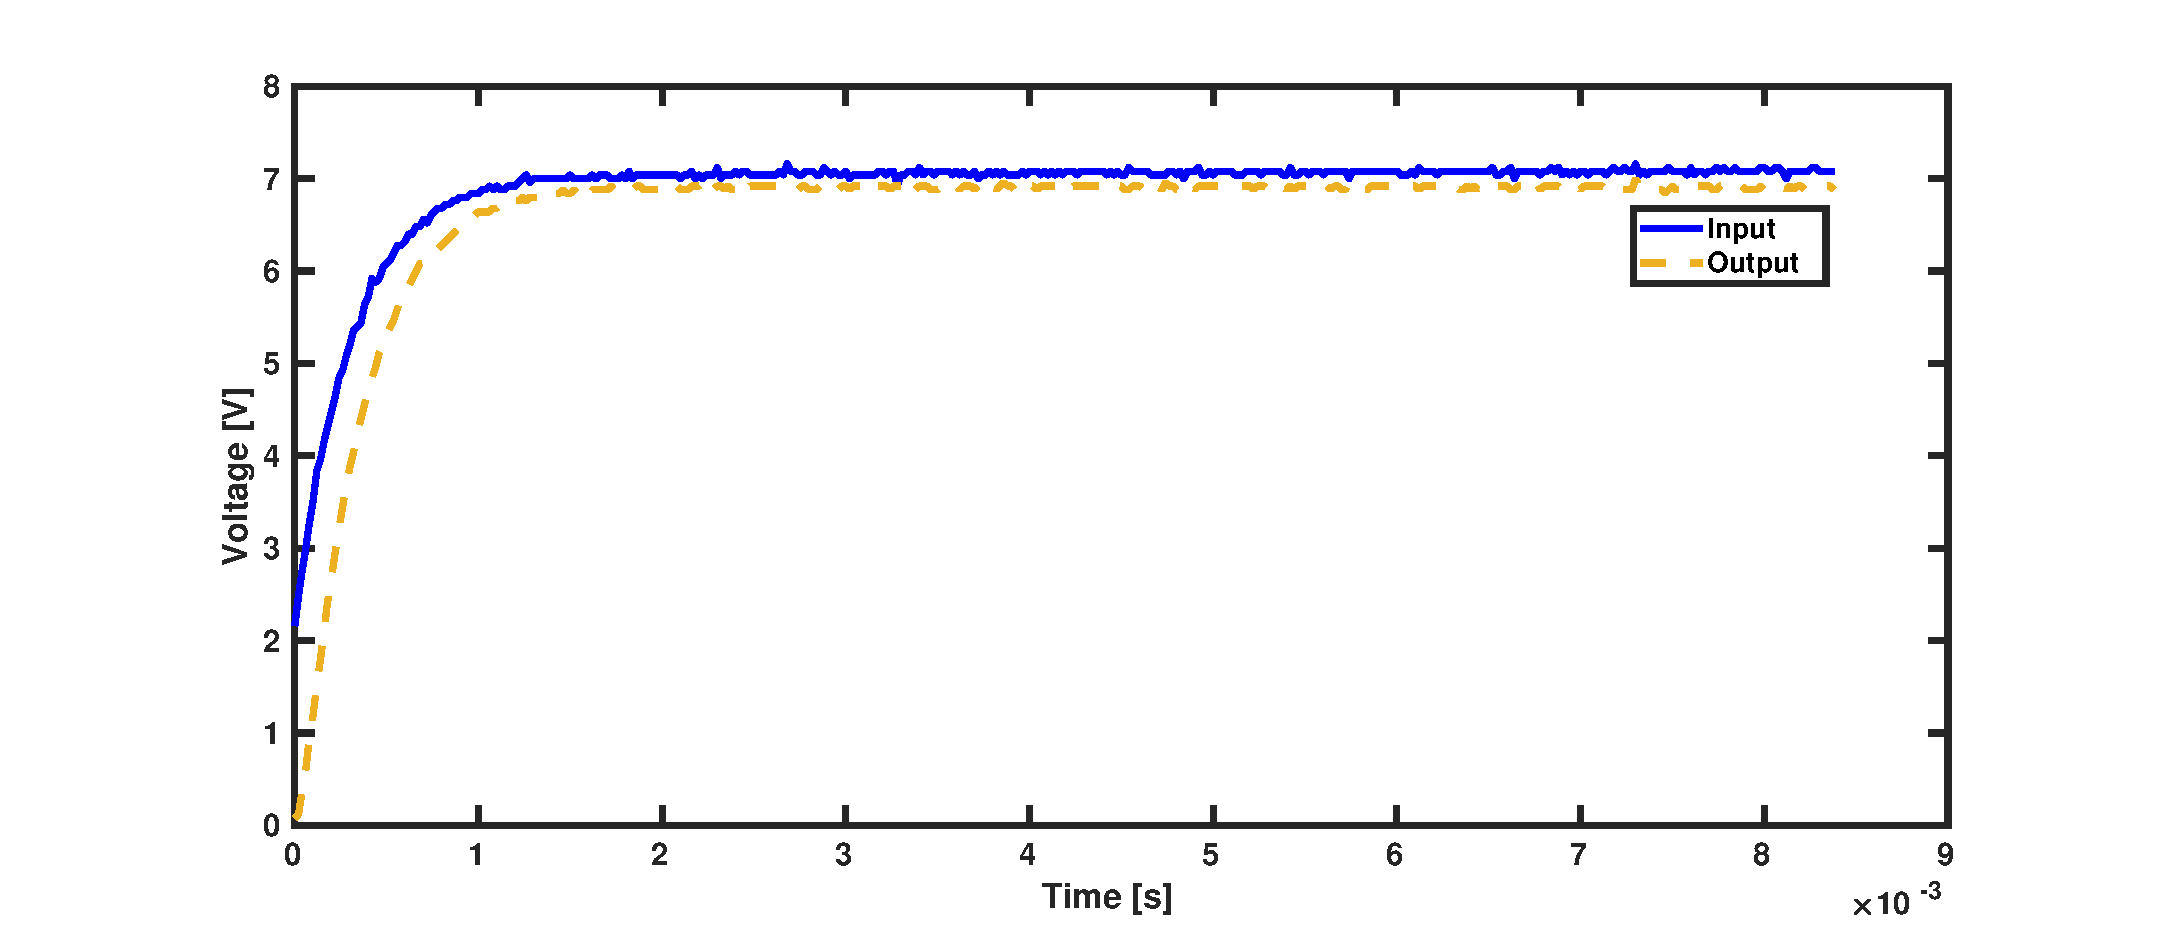
\includegraphics[width=\textwidth]{RmLmDataPlot}
	\caption{Plot of $B_m$ found for each measures}\label{fig:BmTest}
\end{figure}